\documentclass{article}
\usepackage{graphicx}
\usepackage{dirtree}
\usepackage{float}

\title{SSL Project}
\author{Kanak and Harshi}
\date{29 April 2026}

\begin{document}

\maketitle
\tableofcontents
\newpage
\section{Introduction}
This project was made as part of the CS108 (SSL) course in Spring 2026. This game hub is based on royal ancient theme. 
This project applies concepts such as Python, bash, awk, latex, etc. Pygame is used to build GUI for 2D-games.
This Game Hub comprises three mini games, namely-
\begin{itemize}
    \item Tic Tac Toe
    \item Othello
    \item Connect4
\end{itemize}
This project also stores and displays the statistics for each game played by different players.

\section{How to run?}
\textbf{Prerequisites:}
\begin{itemize}
    \item Python should be installed.
    \item Bash commands like dialog must be installed.
    \item Listed modules of pygame must be present.
\end{itemize}
\textbf{Running Instructions:}
\begin{itemize}
    \item Open the repository in the terminal.
    \item Run the main.sh file that will ask for user authentication:\\
    bash main.sh
    \item The main menu of the game will appear after the user authentication, where the players can choose which game to play.
    \item After each game, leaderboard and the respective plots will be displayed.
    \item Afterwards, the players can either replay or quit the game.
\end{itemize}

\section{Hub Structure}
The following is the structure of the directory:
\dirtree{%
    .1 .
    .2 main.sh.
    .2 game.py.
    .2 games.
    .3 tictactoe.py.
    .3 othello.py.
    .3 connect4.py.
    .2 users.tsv.
    .2 history.csv.
    .2 leaderboard.sh.
    .2 Ref\_Images.
    .2 Ref\_Audios.
    .2 report.
    .2 Makefile.
}

\section{Layout}
\begin{itemize}
    \item \textbf{main.sh} Asks for username and password.
    \item \textbf{game.py} Handles the main structure of the Hub. Displays the main menu of game and plots the required graphs.
    \begin{figure}[H]
        \centering
        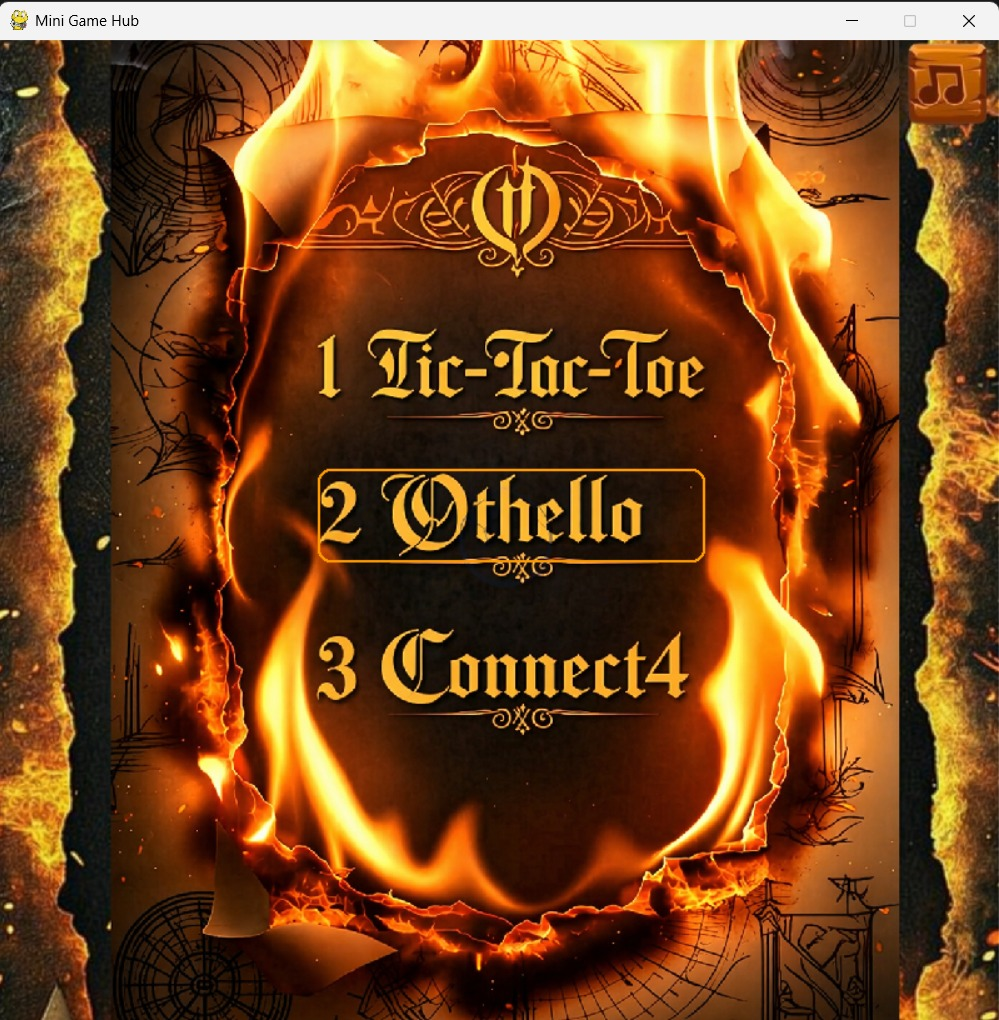
\includegraphics[width=0.5\linewidth]{menu.jpeg}
        \caption{Main Menu}
    \end{figure}
    \begin{figure}[H]
        \centering
        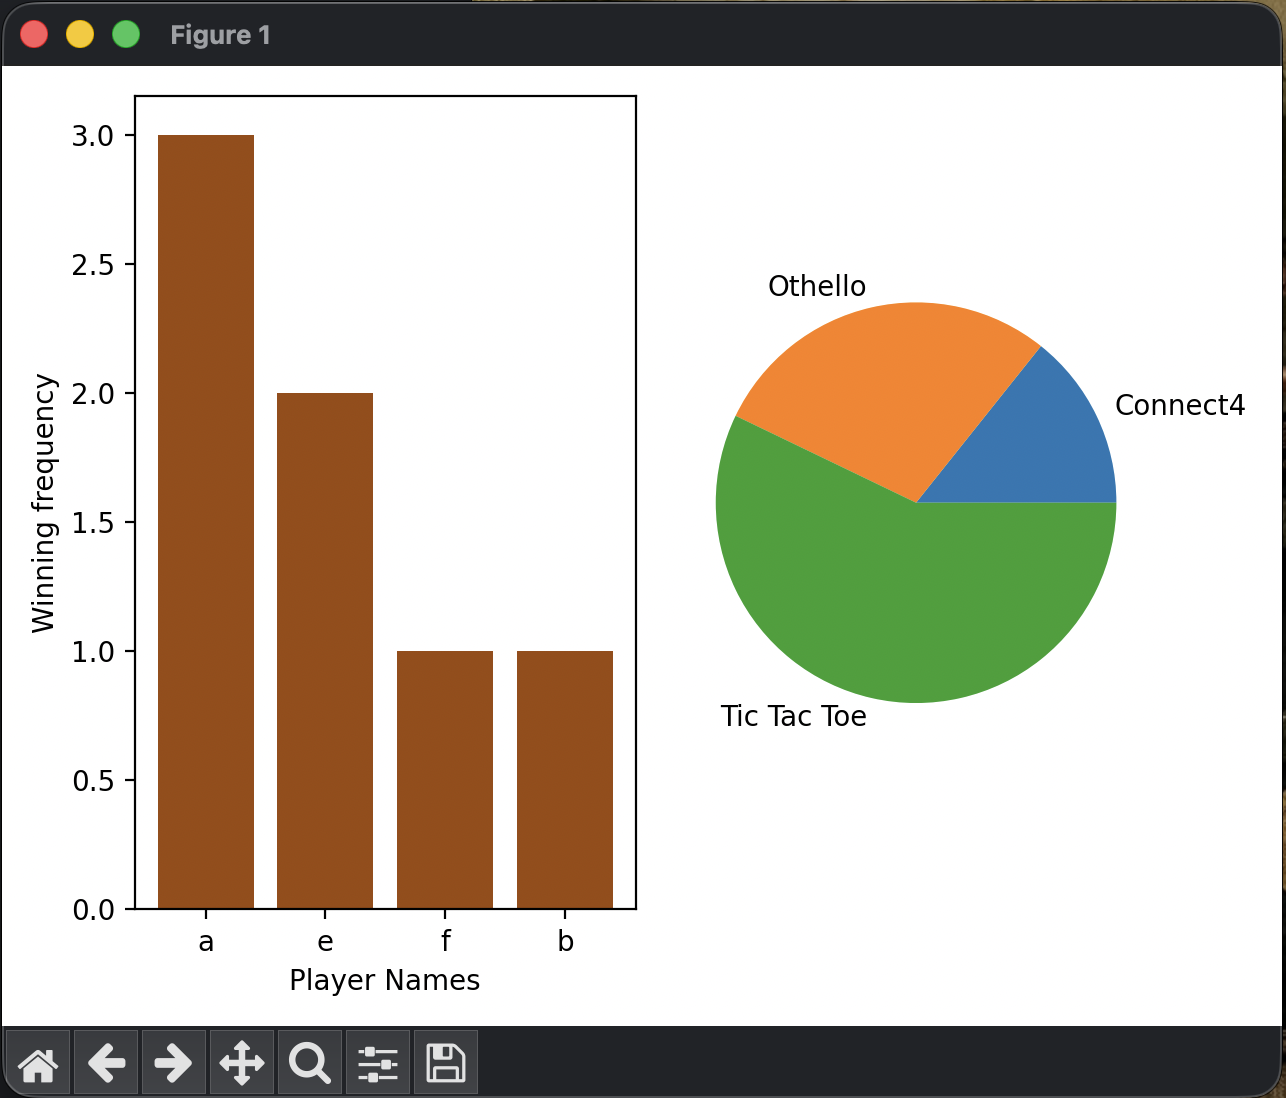
\includegraphics[width=0.5\linewidth]{Statistics.png}
        \caption{Statistics}
    \end{figure}
    \item \textbf{games/} Contains individual games like Tic Tac Toe, Connect4 and Othello.
    \begin{figure}[H]
        \centering
        \includegraphics[width=0.5\linewidth]{TicTacToe.png}
        \caption{Tic Tac Toe}
    \end{figure}
    \begin{figure}[H]
        \centering
        \includegraphics[width=0.5\linewidth]{Othello.png}
        \caption{Othello}
    \end{figure}
    \begin{figure}[H]
        \centering
        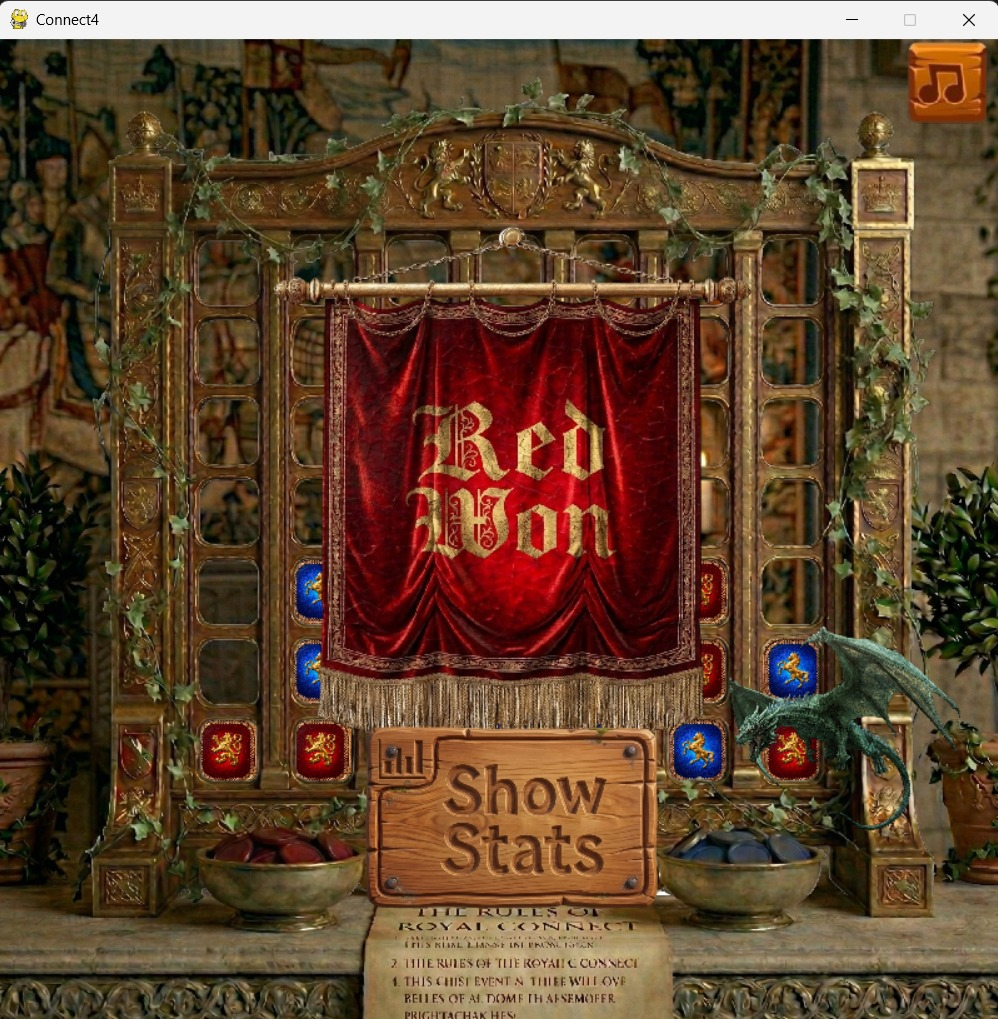
\includegraphics[width=0.5\linewidth]{connect4.jpeg}
        \caption{Connect4}
    \end{figure}
    \item \textbf{users.tsv} Stores the username and passwords for every user.
    \item \textbf{history.csv} Stores the result of each game.
    \item \textbf{leaderboard.sh} Displays the wins and losses of each player per game.
    \begin{figure}[H]
        \centering
        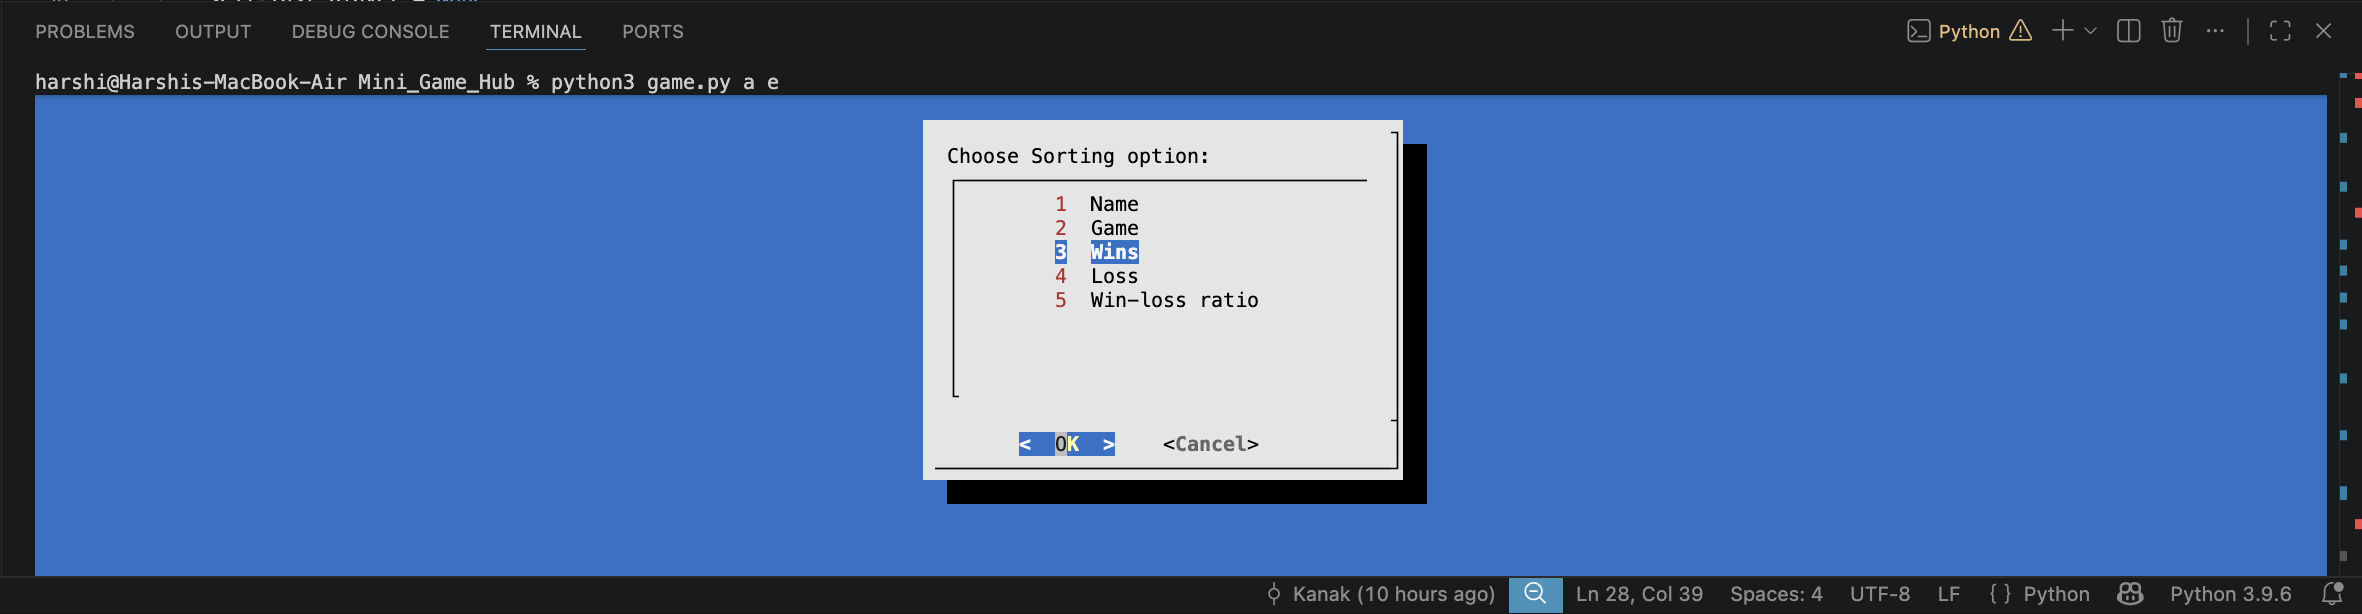
\includegraphics[width=0.5\linewidth]{Leaderboard}
        \caption{Leaderboard}
    \end{figure}
    \item \textbf{Ref\_Images/} Stores all the images used in the games.
    \item \textbf{Ref\_Audios/} Stores the background music of the game.
\end{itemize}

\section{Modules used}
\subsection{Pygame}
Pygame is used for development of minigames. The basic structure of the project i.e, displaying the game, its interface is made up of pygame.

\subsection{NumPy}
NumPy is basically used for mathematical computation in Python. This project uses NumPy to define the board for each individual game and to find the winner.

\subsection{Matplotlib}
Matplotlib is extensively used for visualizing plots in python. It is used in this game to make bar graph and pie chart of top players and frequently played games, respectively.

\subsection{CSV}
CSV module is used to read and write in tabular formatted method written in Comma Separated Files. Here, it is used to add the result of each game to history.csv and extract values from it to make the plots.

\subsection{datetime}
Datetime is used to handle dates and times. It has been used to access the date on which the game is played.

\subsection{sys}
The sys module provides access to variable and functions that interact directly with the system's terminal. It is mainly used here to take the arguments passed by the main.sh which includes the users' name.

\subsection{pathlib}
Pathlib is used to handle the filesystem paths.

\section{Code description}
This project shows an interaction between bash script and python files.\\
The project begins with \textbf{main.sh}. This script:
\begin{itemize}
    \item Prompts the user for authentication (username and password).
    \item Checks credentials using \textbf{users.tsv}.
    \item Passes the authenticated username as an argument to \textbf{game.py}.
\end{itemize}

The \textbf{game.py} file acts as the control center of the game hub:
\begin{itemize}
    \item Displays the main menu using Pygame.
    \item Handles transfer between different games.
    \item Updates \textbf{history.csv} after each game.
    \item Generates graphs using Matplotlib.
\end{itemize}

Each game is made in a separate Python module inside the \textbf{games/} directory:
\begin{itemize}
    \item \textbf{tictactoe.py} Implements a 10x10 grid-based game with turn-based logic.
    \item \textbf{connect4.py} Implements a vertical grid system with gravity-based coin placement.
    \item \textbf{othello.py} Implements board flipping method and detects valid moves.
\end{itemize}

Each game file:
\begin{itemize}
    \item Uses NumPy arrays to make the board.
    \item Handles user input via mouse clicks.
    \item Contains logic for move validation and checking win conditions.
    \item Returns the result (win/loss) to \textbf{game.py}.
\end{itemize}

The \textbf{leaderboard.sh} script:
\begin{itemize}
    \item Reads \textbf{history.csv}.
    \item Computes wins, losses and ratio for each player per game.
    \item Displays the leaderboard in the terminal.
\end{itemize}


\section{Challenges}
\begin{itemize}
    \item \textbf{Handling Class Structure:} Had to avoid circular dependency. Solved by reading documentations and correcting the class structure.
    \item \textbf{Proper motion of coins in Connect4:} Had to do it by first making the motion and then setting the value of the cell to the player.
    \item \textbf{Pause and unpausing the music:} Solved by using the inbuilt pause function of pygame mixer module.
\end{itemize}

\section{Key Understandings}
\begin{itemize}
    \item Basic structure and overview of pygame
    \item Understanding interaction between Bash and Python
    \item Handling CSV files: how to read and write into them
    \item Structure of parent and child classes
\end{itemize}

\subsection{Future Improvements}
If we had more time, we would have added the "TIE" feature of games and would have added different levels in the games. We would have added click sounds.

\end{document}